% %%%%%%%%%%%%%%%%%%%%%%%%%%%%%%%%%%%%%%%%%%%%%%%%%%%%%%%%%%%%%%%%%%%%%
% Header
% %%%%%%%%%%%%%%%%%%%%%%%%%%%%%%%%%%%%%%%%%%%%%%%%%%%%%%%%%%%%%%%%%%%%%

% %%%%%%%%%%%%%%%%%%%%%%%%%%%%%%%%%%%%%%%%%%%%%%%%%%%%%%%%%%%%%%%%%%%%%
% If you want to include a PDF as a first page
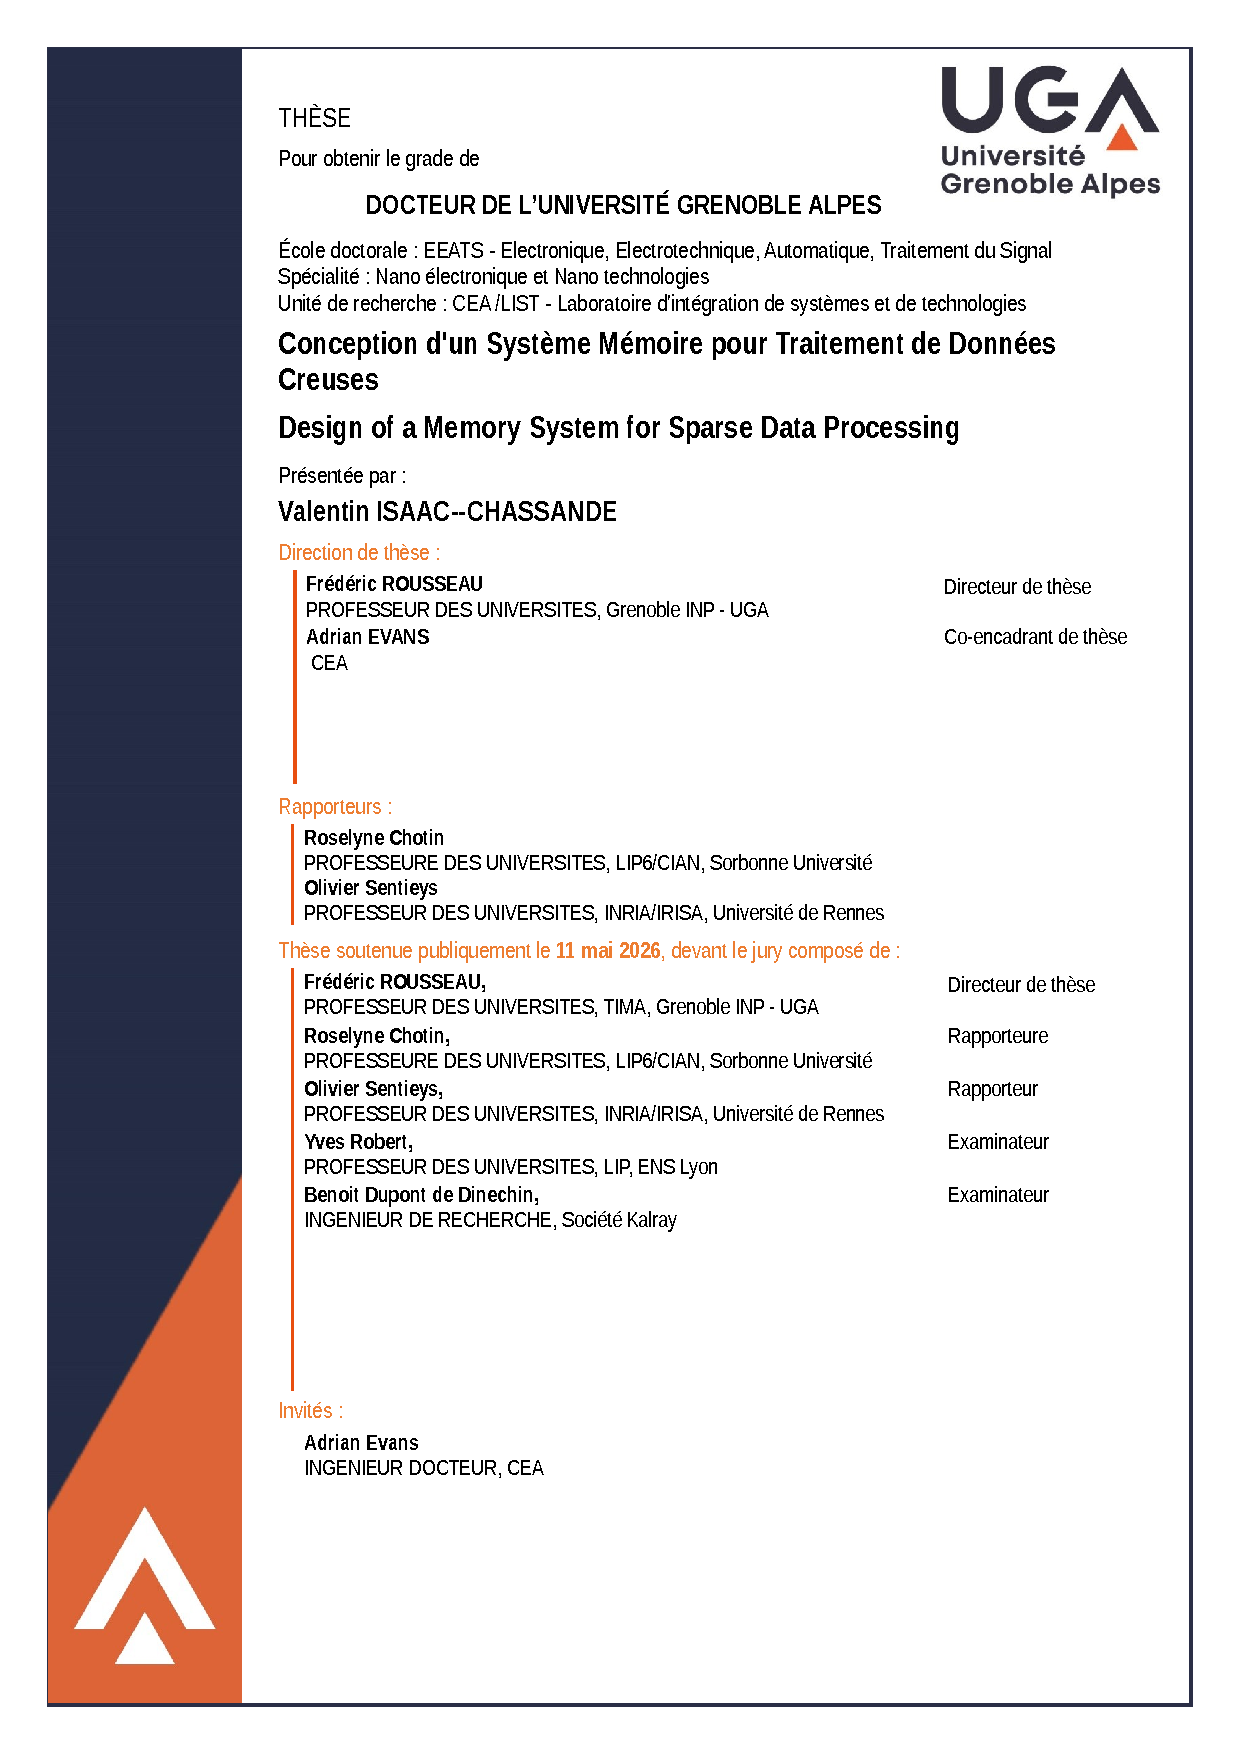
\includepdf[pages=-]{Figures/PDF/couverture_these.pdf}
% %%%%%%%%%%%%%%%%%%%%%%%%%%%%%%%%%%%%%%%%%%%%%%%%%%%%%%%%%%%%%%%%%%%%%

% %%%%%%%%%%%%%%%%%%%%%%%%%%%%%%%%%%%%%%%%%%%%%%%%%%%%%%%%%%%%%%%%%%%%%
% We redefine the title page environment.
% Here is an example of title page:
\begin{titlepage}

%% A A4 PDF to put in the background
% This is just a proposition
% Feel free to modify (you can use the SVGs in Figures/Src as a base)
% See other propositions in Figures/PDF
\ThisULCornerWallPaper{1.0}{Figures/PDF/Fond_Page_de_Garde_CEA-UGA-TIMA}

%% We redefine the page borders. At the end, \restoregeometry is called
%% to go back to the borders defined in Configuration.tex.
\thispagestyle{empty}
\newgeometry{left=1.5cm, right=1.5cm, top=1.50cm, bottom=1.00cm}

\raggedleft
\newlength{\headerheight}
\setlength{\headerheight}{\paperheight-4.5cm}

\begin{minipage}[t][0.2\headerheight]{\linewidth}

    % %% Logos (version with CEA, blanc logos)
    % \raggedleft
    % \newlength{\llogo}
    % \setlength{\llogo}{0.25\linewidth}
    % \begin{minipage}[b][0.5\llogo]{0.12\linewidth}
    %     
\includegraphics[width=\linewidth]{Figures/PDF/LogoBlanc1.pdf}
    %     \vfill
    %     
\includegraphics[width=\linewidth]{Figures/PDF/LogoBlanc2.pdf}
    % \end{minipage}
    % \qquad
    % 
\includegraphics[width=\llogo]{Figures/PDF/LIST.pdf}

    %% Logos (version with CEA, UGA and TIMA)
    \raggedleft
    \newlength{\llogo}
    \setlength{\llogo}{0.25\linewidth}
    \begin{minipage}[b][0.5\llogo]{0.12\linewidth}
        
\includegraphics[width=\linewidth]{Figures/PDF/LogoUGA.pdf}
        \vfill
        
\includegraphics[width=\linewidth]{Figures/PDF/LogoTIMA.pdf}
    \end{minipage}
    \qquad
    
\includegraphics[width=\llogo]{Figures/PDF/LIST.pdf}

    % %% Logos (version with CEA and UGA)
    % \raggedleft
    % \begin{minipage}{0.45\linewidth}
    % 	
\includegraphics[width=0.375\linewidth]{Figures/PDF/LogoUGA.pdf}
    % 	\hfill
    % 	
\includegraphics[width=0.45\linewidth]{Figures/PDF/LIST.pdf}
    % \end{minipage}

\end{minipage}

\centering

\begin{minipage}[t][0.18\headerheight]{\linewidth}
    \normalsize
    \centering

    %% Information about the author. Fill free to add or remove fields
    \textbf{\author}
    	
    Universit\'e Grenoble Alpes
    	
    CEA Grenoble (DRT/LIST/DSCIN/LSTA)
    	
    TIMA Laboratory (SLS)
    
    \textit{ORCID : 0009-0007-9842-5777}
    
    \textit{valentin.isaacchassande@univ-grenoble-alpes.fr}
    
    \textit{valentin.isaacchassande@cea.fr}

\end{minipage}

\begin{minipage}[t][0.08\headerheight]{\linewidth}
    \normalsize
    \centering

    %% The document type defined in Configuration.tex
    \textsc{\doctype}

\end{minipage}

\begin{minipage}[t][0.12\headerheight]{\linewidth}
    \normalsize
    \centering

    %% The title defined in Configuration.tex
    \begin{minipage}{16cm}
        \centering
        \begin{spacing}{2}
    	    \textbf{{\LARGE \textsc{\title}}}
    	\end{spacing}
    \end{minipage}

\end{minipage}

\begin{minipage}[t][0.12\headerheight]{\linewidth}
    \normalsize
    \centering

    %% Date (automatic with that command)
    \today

\end{minipage}

\begin{minipage}[t][0.23\headerheight]{\linewidth}
    \normalsize
    \centering

    %% Some supervisor names (example of a thesis)
    \begin{tabular}{rl}
        Thesis Adviser: & Fr\'ed\'eric ROUSSEAU \\
        Thesis Co-Supervisors: & Adrian EVANS \\
        & Yves DURAND \\
        & \\
        CSI Members: & Yves ROBERT (HDR) \\
        & Christophe PICARD
    \end{tabular}

\end{minipage}

\begin{minipage}[b][0.07\headerheight]{\linewidth}
    \normalsize
    \centering

    %% Any Additional Information
    EEATS Doctoral College, NENT Speciality
    
    \StartYear~-- \EndYear~Academic Years
    
    From \StartDate~to \EndDate

\end{minipage}

\end{titlepage}
% %%%%%%%%%%%%%%%%%%%%%%%%%%%%%%%%%%%%%%%%%%%%%%%%%%%%%%%%%%%%%%%%%%%%%

\restoregeometry